
%[Some intro of Jazz repository]

% Commenting on work items is the main task-related communication and collaboration
% channel used by \jazztm\ developers. Work items represent single
% assignable and traceable tasks and a set of work items defines the tasks for each
% team in each iteration. Different types of work items represent defects,
% enhancements, user stories, and general tasks. The work items are assigned to,
% and owned by, project participants. The coordination that is necessary for the
% implementation of the work items is facilitated by work item collaboration
% behavior that includes contributors to comment or observe the communication
% around work items, by being subscribers to the work item.

\section{Social Network Analysis with \jazztm}

We applied our approach to mine and construct social networks with the IBM
Rational \jazztm\ project in several research studies. First, we describe how
\jazztm\ concepts and artifacts were mapped to the concepts used in our general
approach. Then, we describe our data mining tools, followed by two research
studies conducted using data extracted from the \jazztm\ development project.

IBM Rational is building \jazztm\ \cite{Frost:2007ff} as a scalable and
extensible team collaboration platform for integrating development work across
task, build, source code, and planning management activities. \jazztm\ is
developed by a globally distributed team that uses \jazztm\ to manage its own
work. The \jazztm\ platform uses a client-server architecture, where the server
is the central data repository that stores data for \jazztm\ components. The
repository is accessible using a web-based client interface or an Eclipse-based
client. Our elements for constructing social network map to Jazz artifacts as
follows:

\begin{description}
\item[Project Members] are \emph{contributors} in Jazz.
Personal information, such as the name and email address of each contributor, as well as
project related information, such as team affiliations are available.

\item[Collaborative Tasks] are \emph{work items} in Jazz. Work items represent
the basic unit of work in \jazztm\ and can describe many types of tasks such as
bug reports, modification requests, or development tasks. Work items have a
comment-based conversation, a list of observing subscribers, and other attributes
such as, a creation date, a description, and an owner.

\item[Task-related Communication] is \emph{comments} on work items in Jazz.
Reading and writing comments on work items is the main collaboration mechanism in
Jazz as developers use comments to debate and discuss decisions. A thread of
comments forms a conversation that is attached the work item. Each comment
has a creation date, comment text, and an authoring contributor.

\end{description}

% XXX -- fix my location
\begin{figure*}[tb]
\begin{center}
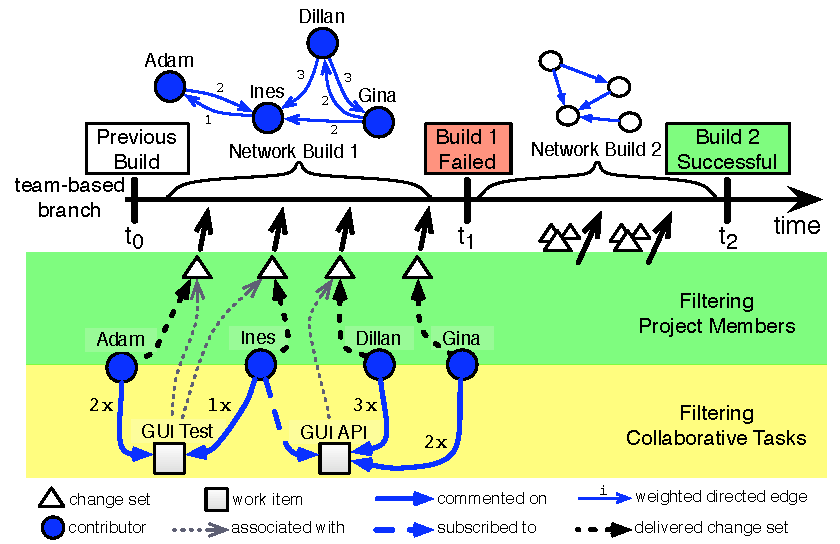
\includegraphics[width=1.3\columnwidth]{./figures/BuildResultNetworks}
\caption{Construction of social networks for build failure prediction}
\label{fig:BuildSNs}
\end{center}
\end{figure*}

\subsection{Data Mining Tools for \jazztm}
In order to extract the elements needed to construct and analyze social networks,
we implemented several data mining and social network analysis tools. To extract
data of interest, we developed a plug-in for the Eclipse-based \jazztm\ client
that used the provided Java API to query and retrieve the desired data from the
repository.

The \jazztm\ development project has a large \jazztm-based repository containing
more than 40,000 work items, 150 contributors, and 5,000 build results. We
needed to collect data from the live development repository without affecting the
\jazztm\ development team's server performance, potentially disrupting their
work. To meet this goal, we designed our data extraction tool to be minimally
invasive and to use incremental queries, extracting small portions of the data
set at a time, to minimize performance degradation.

Further, the querying and processing of the extracted data to construct social
networks is an additional challenge because it is data and time intensive. For
example, extracting and processing all work items from the repository took
several hours. Thus, it is not feasible to extract and process all of the
information needed to construct social networks in real-time. For this reason, we
import the data of interest into a reporting and analysis database. This approach
allowed us to use a large proportion of the data in the \jazztm\ team's
repository for social network construction and analysis without adversely
affecting their development environment.

% Each data type's external XML file representation is independent so that a single
% query result can already be used for analysis, without requiring all associated
% data types or associations. For example, when only exporting the work items that
% were created or modified during a specific week, the resulting data file can
% already be analysed without the need of any associated data types like the
% contributors. In addition, data and associations between data types that result
% from subsequent queries can be added without changing the previous extracted
% information. This data structure enables us to mine large data sets in many small
% through incremental queries without affecting the Jazz server repository.

To process the data from the database we used the Java Universal Network/Graph
Framework (JUNG) to construct and visualize the task-based social networks and to
compute social network analysis measures. Our tools also generate data sets for
use as inputs to other tools, such as statistical analysis using the R language,
or social network analysis using UCINET.

%\paragraph{Filter Project Members}
%\ \\
%In \jazztm\ we filter \people s by different criteria to focus on people to meet
%each collaboration scope. One way to do that would be to focus on all people that
%made changes to the source code included in a build. For that we would identify
%all chances made for that build and identify the people that made those changes.

%\paragraph{Filter Collaboration Tasks}
%\ \\
%One major task during the \jazztm\ development would be to deliver a successful
%build of \jazztm. Our XXX would focus on a build within \jazztm\ and only include
%work items that are build related. In addition, the XXX would define the time
%frame starting on the previous build and the build of interest.

%\paragraph{Connect Project Members}
%\ \\
%Contributors comment on work items to ask questions, debate descisions, or to
%provide additional information, such as screenshots. A series of comments on a
%work item forms a conversation thread. When connecting \people s while
%constructing our social networks, we connect those who have commented on a work
%item, as we assume that they have exchanged information and thus communicated.
%Additionally, we assume that subscribers of a work item listen to the
%communication, but have not actively contributed. We also include the creator of
%the work item as a contributor because a work item's initial description is the
%start of the conversation.

% The communication between two \people s is directed, since participating in a
% work item conversation thread means sending and receiving information. Whereas,
% subscribing to a work item only provides one-way communication, so directed edges
% are used to connect \people s. Weights can also be applied to communication links
%  by using the number of comments exchanged between two \people.


\subsection{Research Studies Using Social Network Analysis}
We used the mined task-based social networks in two of our research studies that
map to the more general build failure \cite{wolf:tr2008} and communication
broker \cite{Nguyen:2008Distance} examples provided earlier.

\paragraph{Communication Structures to Predict Build Failures}
\ \\
In this study we were interested in investigating whether properties of an
integration team's social network have any relationship with the integration
outcome. Code integrations (referred  to  as builds in Jazz)  are frequent and
very important in the Jazz project. The continuous integration process requires
regular daily and weekly integrations of each team's work into an assembled
product. A build can succeed or fail due to compilation, testing, or other
integration errors.

To integrate in \jazztm, the members of a development team commit source code
changes (change sets) to a team-based branch. Each change set is associated with
the work item that describes the change it implements, and contributors comment
on the work items to discuss the changes. As such, the \emph{collaboration scope}
of this study is the communication of contributors who have delivered change sets
that were included in each build. 

%DD. Shortened the text to avoid repeition from section 1, as per comment #2

To construct the social networks for Build 1 at time t$_1$ (as illustrated in
Figure~\ref{fig:BuildSNs}), we followed the steps outlined in our Failed Build
example described earlier: we filtered the contributors that delivered change
sets between t$_0$ and t$_1$ and identified all work items that were associated
with code change sets in Build 1. To connect contributors in the social network
we add a directed edge between each pair of contributors who have either
commented or subscribed to a common work item since the last build. The weight on
directed edges represents the number of comments on the shared work items.

% T.W. Changed the following paragraph to address point 3 from revision 2
After we constructed the social networks for each integration build of the five
teams
% R3.2
(between 48 and 60 builds for each team), we computed different social network
measurements, such as \emph{centrality}, \emph{betweenness}, and
\emph{density}~\cite{Wasserman:1994dz} and investigated their relationship to
integration outcomes. Although none of these measures can independently predict
the build outcome, when used in combination they are more powerful. We developed
a predictive model by training a
% R2.4
Bayesian classifier that was able to accurately predict failed build results. The
recall and precision values of the predictions using measures of social network
structure is shown in Table~\ref{tab:predictionResults} for the five teams.
% R3.2
In order to validate our model for each of the five teams we used \emph{leave one
out cross validation}, which trains a model for each set of data points that is
in size one smaller then the full set, and then predicts the data point that is
not in the training set. Study details are available in technical
report~\cite{wolf:tr2008}.

\begin{table}
\small
\begin{tabular}{r|c c c c c|c}
\hline
  & \multicolumn{5}{c|}{Teams} & Std.Dev. \\ \hline
Recall 		& 55\% & 75\% & 62\% & 66\% & 74\% & 8.38\% \\ 
Precision 	& 52\% & 50\% & 75\% & 76\% & 66\% & 1.34\% \\ \hline
\end{tabular}
\caption{Prediction results for the five teams}
\label{tab:predictionResults}
\end{table}


% R2.4 NOTE FROM DANA: NO NEED TO HAVE THIS NEXT PARA, SO I COMMENTED IT. THE
% REVIEWER WAS JUST BEING VERY TOUGH.. 
% Although, the results are compared to a general failure probability of 50\%, we
% consider this result as a first step towards indicating that communication
% influence source code quality.


\paragraph{Communication Structures in a Large Distributed Project}
\ \\
In this second study \cite{Nguyen:2008Distance} we were interested in the
project-wide communication structure of the geographically distributed \jazztm\
development team. A quantitative analysis of response time for task
communication and task resolution times revealed a lower than expected impact of distance on these
factors. We explored the project's social networks for useful insights that might
explain this effect. Specifically, we were interested in identifying properties
of the social networks, such as cohesiveness of the distributed teams, that were
related to the results of communication delay and distributed collaboration.

The \emph{collaboration scope} of this study is the entire project, and thus
includes all collaborative tasks, and all contributing project members. In this
case, connecting project members is the key step to create a project-wide social
network. 

%DD shortened the text to address comment #2. 
To construct the project-wide social network we followed the steps as
exemplified in Section 1.3 (the communication broker example).


The resulting social network is illustrated in Figure~\ref{fig:JazzProjectSN} in
which ovals indicate the teams at each geographic site. We used the \emph{k-core}
and \emph{core-periphery} tests \cite{Wasserman:1994dz} to analyze the properties
of the network structure. These tests allowed us to test whether multiple
cores can be identified in the network, or the network shows a star-like 
structure in which a single core mediates communication with the developers on
the periphery of the network.
%R3.5 && R2.5

The results indicate that the project-wide team collaborates as a cohesive team
with one large core, as opposed to many loosely connected clusters. The colors in
the figure illustrate how close a team member is to the core of the whole
project. In red we show a core of active developers (60 of
112 project members) where each developer
communicates with at least other 25 developers from the core. The other
colors, from yellow to light blue, indicate different lower degrees of communication in
the project. Further, using the
\emph{group degree centrality} \cite{Wasserman:1994dz} measure, we also found
that each geographic location has roughly equal centrality and used the people in
the core to stay connected to the rest of the large team. This means that project
members communicate well with project members at each other geographic location.
This may explain why distance had an insignificant effect on communication response
and task resolution time in the large distributed team.

% R3.2
In summary, we learned from this study that communication delay as a result of
distribution in global teams can be overcome with recent
collaboration tools and practices. From our experience with the Jazz team, best practices such as prioritizing
off site requests and tools that integrate development, project
management and communication play a major role in achieving these results.

\begin{figure}[t]
\begin{center}
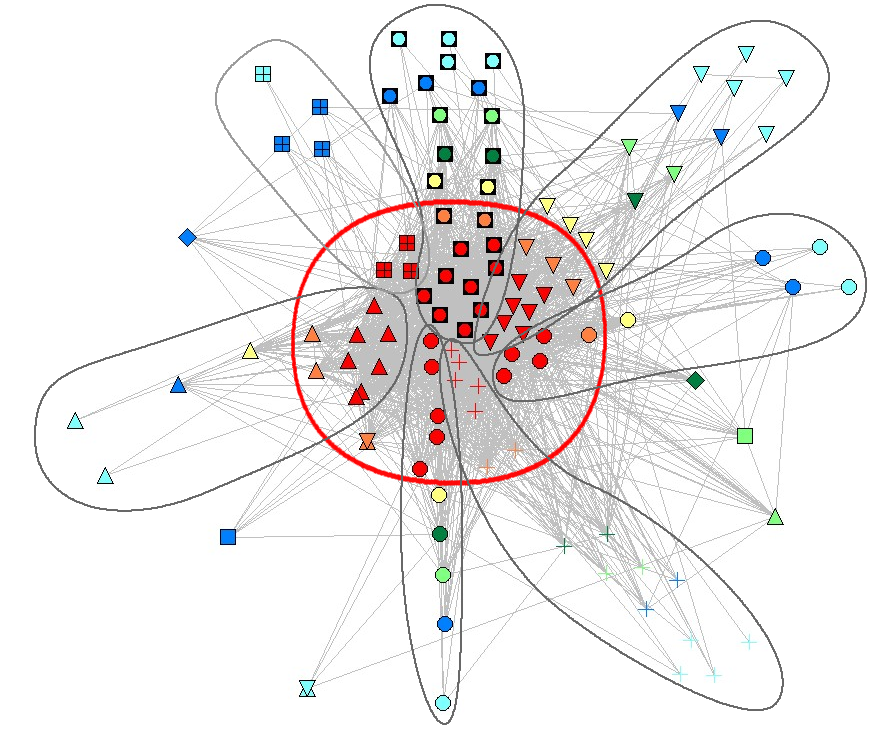
\includegraphics[width=0.99\columnwidth]{./figures/JazzProjectSN}
\caption{Project-wide communication-based social network}
\label{fig:JazzProjectSN}
\end{center}
\end{figure}

% ~\cite{Seidman:1983sn}
 % ~\cite{Borgatti:2000kl}
% ~\cite{Everett:2005dn} Details are published


